\documentclass[xetex]{beamer}


\mode<presentation> {
%  \usetheme{Singapore}
  \usetheme{Frankfurt}
  \setbeamercovered{transparent}
}

\usepackage{xunicode}
\usepackage{xltxtra}
\usepackage[czech]{babel}
\usepackage{palatino}
\usepackage{graphicx}
\usepackage{tikz}
\usepackage{pgflibraryarrows}
\usepackage{pgflibrarysnakes}

\title{Úvod do světa\\ operačních systémů}

\author{Ondřej Profant}
\institute[Piráti]{Knihovna Průhonice\\ Česká pirátská strana}
\date{\today}

\begin{document}

\begin{frame}
  \titlepage
\end{frame}

\begin{frame}
  \frametitle{Osnova}
  \tableofcontents
\end{frame}	

\section{Co to je operační systém?}

\subsection{Definice poprvé}
\begin{frame}
 \frametitle{Co to je operační systém?} 
\begin{block}{Definice}
Operační systém je v informatice základní programové vybavení počítače (tj. software), které je zavedeno do paměti počítače při jeho startu a zůstává v~činnosti až do jeho vypnutí. Skládá se z~jádra (kernel) a pomocných systémových nástrojů. Hlavním úkolem operačního systému je zajistit uživateli možnost ovládat počítač, vytvořit pro procesy stabilní aplikační rozhraní (API) a~přidělovat jim systémové zdroje. Operační systém je velmi komplexní software, jehož vývoj je mnohem složitější a~náročnější, než vývoj obyčejných programů.
\end{block}
 \begin{flushright}
  Wikipedie
 \end{flushright}
\end{frame}

\subsection{Hardware}
\begin{frame}
 \frametitle{Hardware}
  \begin{itemize}
  \item Fyzická část počítače
  \item Tzv. železo`
 \end{itemize}
 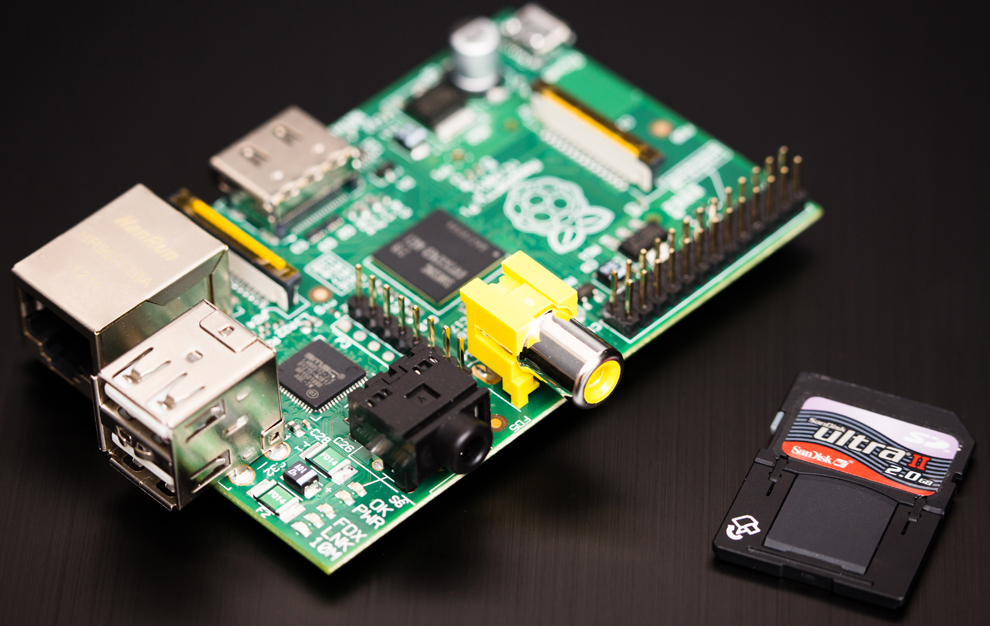
\includegraphics[scale=0.25]{pic/hw.png}
\end{frame}

\subsection{Software}
\begin{frame}
 \frametitle{Software}
 \begin{itemize}
  \item Jednotlivé aplikace (kalkulačka, internetový prohlížeč, malování, \ldots{}).
  \item Aplikace nedělá vše. Pro spoustu věcí/činností potřebuje připravenou infrastrukturu. 
 \end{itemize}
\end{frame}

\subsection{Definice podruhé}
\begin{frame}
 \frametitle{Co to je operační systém?}
 \begin{itemize}
  \item Nejnižší úroveň SW (aplikací)
  \item Pracuje přímo s HW (železem)
  \item Prostředník mezi HW a SW
 \end{itemize}
\end{frame}


\section{Stručná historie}

\begin{frame}
 \frametitle{Stručná historie}
 \begin{itemize}
  \item Původně byl operační systém svázán s konkrétním strojem
  \item Až postupem času se začaly stávat univerzální počítače (dnes je univerzalita největší výhod)
  \item Původně jsou počítače silně provázány s~armádou i~s~akademickou sférou
 \end{itemize}
\end{frame}

\subsection{Časová osa}
\begin{frame}
 \frametitle{Časová osa}
 \begin{scriptsize}
 \begin{tikzpicture}
  \def\osaA{9};
  \def\osaAlabel{8.7};
  \def\osaB{5};
  \def\osaBlabel{4.7};
  \draw (0,\osaA) -- (10 , \osaA);
  \draw (1,\osaAlabel) 	node{ \ldots{}	};
  \draw (3,\osaAlabel) 	node{ 17. stol.	};
  \draw (5,\osaAlabel) 	node{ 18. stol.	};
  \draw (7,\osaAlabel) 	node{ 19. stol.	};
  \draw (9,\osaAlabel) 	node{ \ldots{}	};
  \draw (0,\osaB) -- (10 , \osaB);
  \draw (0,\osaBlabel) 	node{1900};
  \draw (0.7,\osaBlabel) 	node{\ldots};
  \draw (2,\osaBlabel) 	node{1940};
  \draw (4.5,\osaBlabel) 	node{1960};
  \draw (7,\osaBlabel) 	node{1980};
  \draw (9.5,\osaBlabel)	node{2000};
  %
  \draw  (1,\osaA+1) node[rotate=60]{Abakus};
  \draw  (3,\osaA+1) node[rotate=60]{Pascalina};
  \draw  (7.0,\osaA+1) node[rotate=60]{Charles};
  \draw  (7.4,\osaA+1) node[rotate=60]{Babbage};
  %  
  \draw  (1.2,\osaBlabel-0.3) 	node{38};
  \draw  (1.2,\osaBlabel+1) 	node[rotate=60]{Z1};
  \draw  (2.2,\osaBlabel-0.3)   node{43};
  \draw  (2.05,\osaBlabel+1) 	node[rotate=60]{Colossus};
  \draw	 (2.2,\osaB) -- (2.2,\osaB+0.3);
  \draw  (2.5,\osaBlabel)   	node{44};
  \draw  (2.5,\osaBlabel+2.1) 	node[rotate=60]{EINIAC};
  \draw	 (2.5,\osaB-0.14) -- (2.5,\osaB+1.3);
  \draw  (2.8,\osaBlabel-0.3) 	node{47};
  \draw  (2.9,\osaB+1) 			node[rotate=60]{tranzistor};
  \draw  (3.1,\osaBlabel) 		node{50};
  \draw  (3.1,\osaBlabel+1)		node[rotate=60]{Z4};
  \draw  (3.7,\osaBlabel-0.3) 	node{57};
  \draw  (3.7,\osaBlabel+1)		node[rotate=60]{SAPO};
  \draw	 (3.7,\osaB-0.3) -- (3.7,\osaB+0.4);
  \draw  (4.8,\osaBlabel-0.3) 	node{65};
  \draw  (4.9,\osaBlabel+2.15)	node[rotate=60]{IBM 360, UNIX};
  \draw	 (4.75,\osaB) -- (4.75,\osaB+1.3);
  \draw  (5.2,\osaBlabel) 		node{69};
  \draw  (5.2,\osaBlabel+1.5)	node[rotate=60]{ArpaNET};
  \draw  (5.7,\osaBlabel-0.3) 	node{71};
  \draw  (5.7,\osaBlabel+1.5)	node[rotate=60]{mikroprocesor};
  \draw	 (5.7,\osaB-0.4) -- (5.7,\osaB+0.6);
  \draw  (8,\osaBlabel-0.3) 	node{89};
  \draw  (7.9,\osaBlabel+0.9)		node[rotate=60]{www};
  \draw	 (8,\osaB-0.3) -- (8,\osaB+0.3);
  \draw  (8.5,\osaBlabel)	 	node{91};
  \draw	 (8.5,\osaB) -- (8.5,\osaB+1);
  \draw  (8.5,\osaBlabel+1.6)	node[rotate=60]{Linux};
  \draw  (9,\osaBlabel-0.3) 	node{94};
  \draw	 (9,\osaB-0.4) -- (9,\osaB+0.65);
  \draw  (9.2,\osaBlabel+1.7)		node[rotate=60]{komerč. internet};
  \draw	 (9,\osaB) -- (9,\osaB+0.8);
 \end{tikzpicture}
 \end{scriptsize}
\end{frame}

\subsection{Zajímavosti}


\begin{frame}
 \frametitle{Zajímavosti - Abakus též počítadlo} 
 Abakus je prokázán již 3000 př. n. l.
 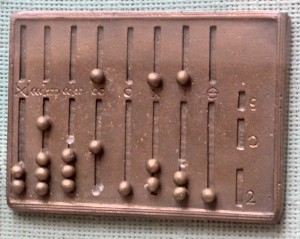
\includegraphics[scale=0.9]{pic/abakus.jpg}
\end{frame}

\begin{frame}
 \frametitle{Zajímavosti - Pascalina}

 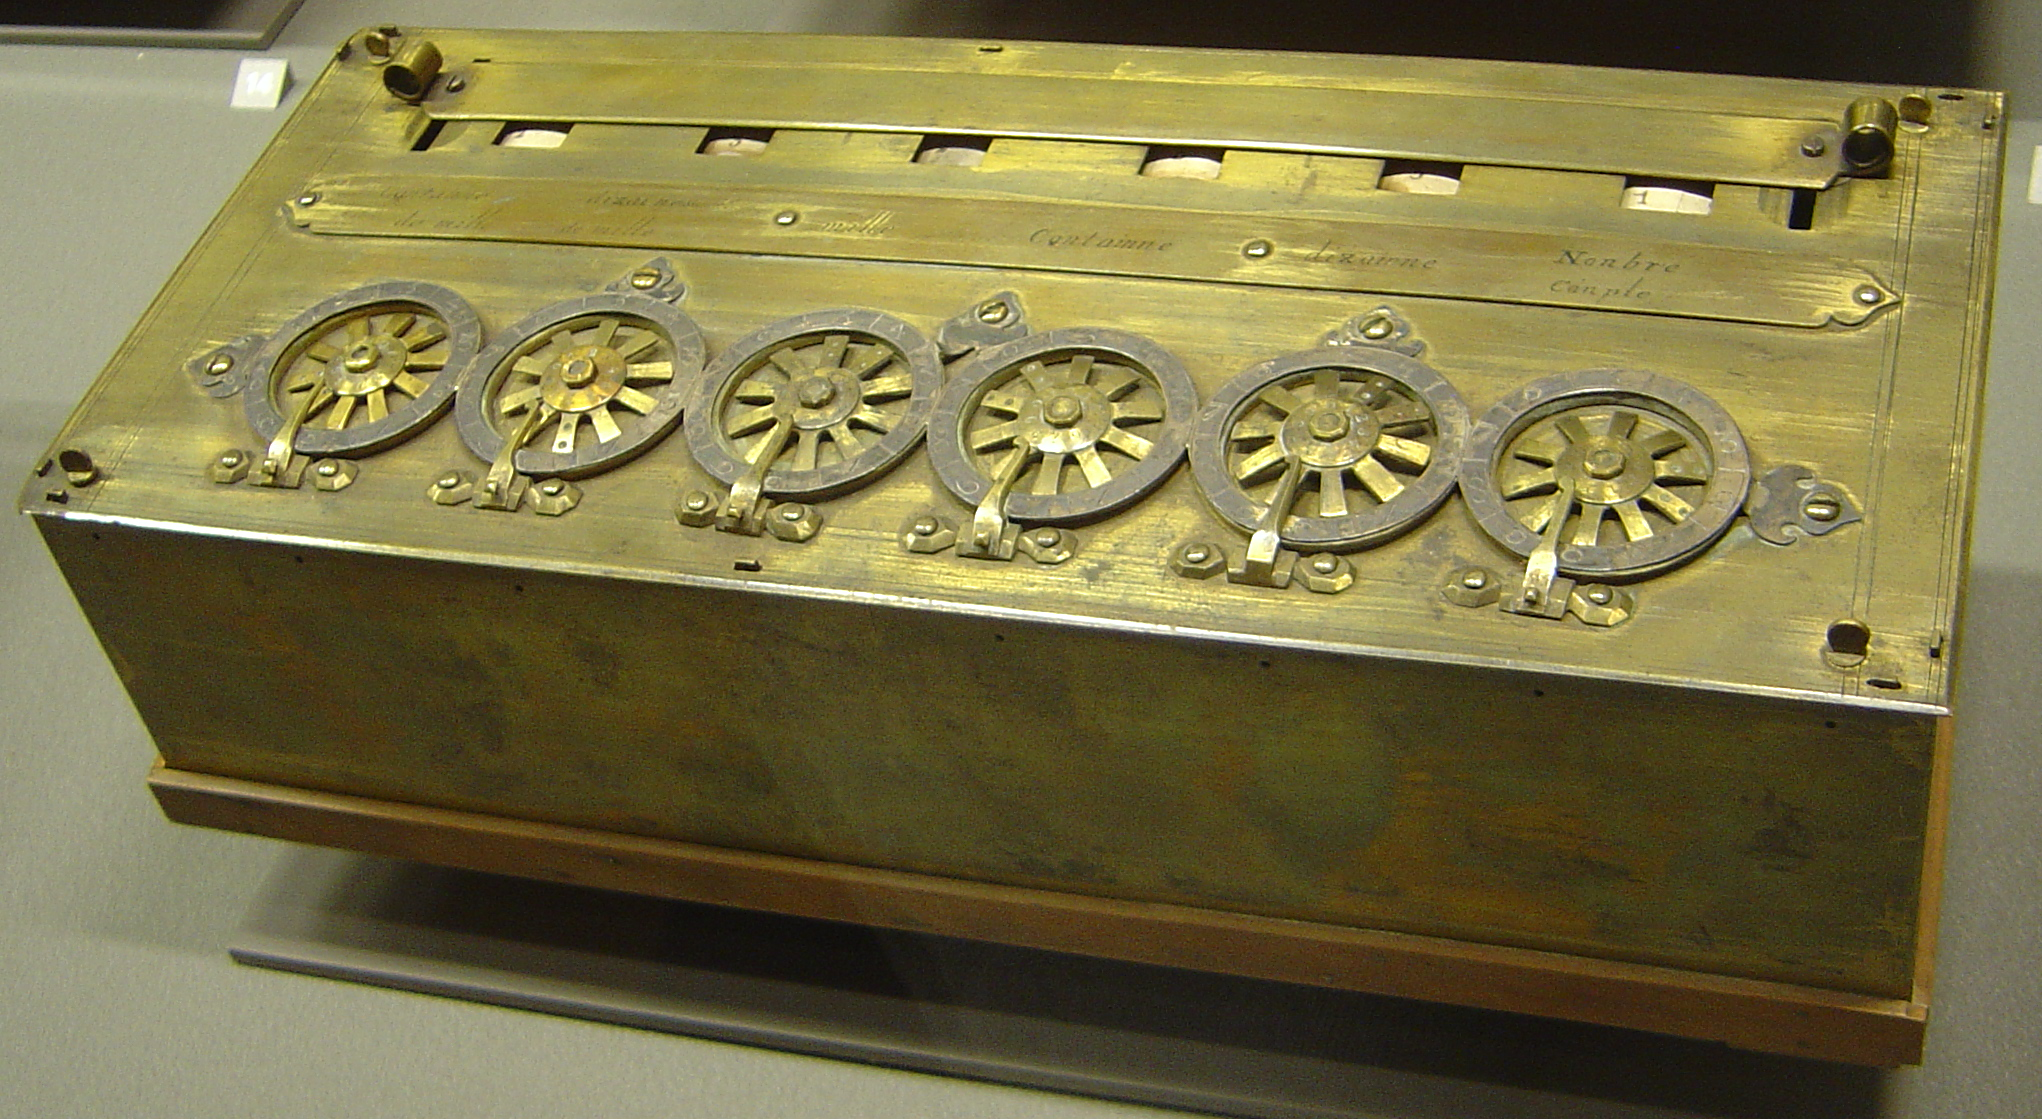
\includegraphics[scale=0.17]{pic/pascalina.jpg}
\end{frame}


\begin{frame}
 \frametitle{Zajímavosti}
 \begin{itemize}
 \item Charles Babbage navrhl plně programovatelný počítač v~roce 1837.
 
 Ke konci 20. století byl počítač sestaven a shledán funkčním.
 
 \item Počítače Konráda Zuseho se používali velmi dlouho (např.~švýcarské banky).
 \item Linux vznikl proto, aby jeho autor (Linus Torvalds) mohl testovat software bez drahého komerčního UNIXu.
 \end{itemize}
\end{frame}

\section{Taxonomie}
\begin{frame}
 \frametitle{Taxonomie operačních systémů}
 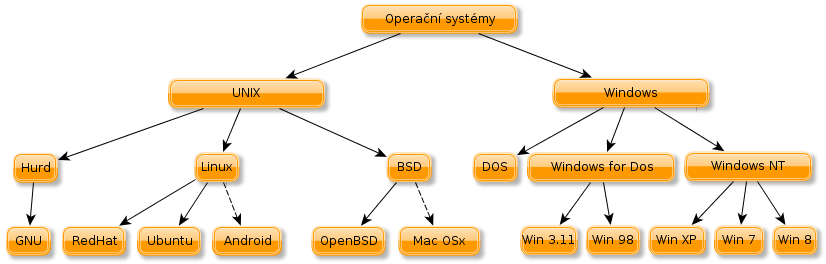
\includegraphics[scale=0.39]{pic/os.png}
\end{frame}

\section{Závěr}
\subsection{Zdroje}
\begin{frame}
 \frametitle{Zdroje}
 \begin{itemize}
 \item Přednáška Úvod do operačních systémů na MFF UK
 \item Komunita: wikipedie.cz , hesla:
 \begin{itemize}
  \item Tranzistor
  \item Počítadlo
  \item Operační systém
  \item Unix
 \end{itemize}
 \item Komunita: wikipedia.org , hesla:
 \begin{itemize}
 \item Charles Babbage
 \item Pascalina
 \end{itemize}
 \item Ondřej Profant: Kurz základní práce s počítačem\\ (doplňující text k~výuce, zde v knihovně)
 \end{itemize}
\end{frame}
\subsection{Diskuse}
\begin{frame}
  \frametitle{Závěr}
	Děkuji za pozornost.

	\bigskip
	
	Doplňující otázky?

\bigskip

\bigskip

\scriptsize
Copyleft Ondřej Profant, 2012. Všechna práva vyhlazena. Sdílejte, upravujte a~nechte sdílet za stejných podmínek. 

Prezentace v~úplné formě\footnote{i se zdrojovými kódy} na vyžádání emailem: ondrej.profant -at- pirati.cz 
\end{frame}
\end{document}
